\section{Результаты измерений и обработка данных}

\subsection{Изучение работы оптического пирометра}

С помощью пирометра и при помощи термопарного термометра измерена температура модели АЧТ. Проверим корректность измерений: температура на пирометре не должна сильно отличаться от температуры АЧТ, измеренной термопарой. Температура, измеренная пирометром, составила $t = 1062^{\circ}$С, измеренная при помощи термопары~-- $t = 1060^\circ$C. Разница составляет менее 0,2\%, что позволяет нам утверждать, что измерения при помощи пирометра достаточно достоверны. 

\subsection{Измерение яркостной температуры тел}
Качественно проверено, что разные тела, накалённые до одинаковой термодинамической температуры, могут иметь различную яркостную температуру. Для этого несколько образцов из разных материалов было нагрето до одинаковых термодинамических температур. Яркостная температура поверхности образцов~-- трубки и колец~-- оказалась примерно следующей:
    \begin{itemize}
        \item Керамическая трубка: 750-800 $^{\circ}$C;
        \item Металлические кольца: $\approx$ 750 $^{\circ}$C; 
        \item Неметаллические кольца $<$ 700 $^{\circ}$C (не определяется пирометром).
    \end{itemize}
Несовпадение яркостной температуры у различных тел, имеющих одинаковую термодинамическую температуру, возникает из-за того, что эти две величины связаны, в том числе, через спектральный коэффициент поглощения, который у разных материалов различный.    

\subsection{Проверка закона Стефана-Больцмана}
В диапазоне 900-1900 $^\circ$C измерена яркостная температура нити лампы накаливания, а также значение силы тока и напряжения на ней. Определим также по значениям яркостной температуры нити её термодинамическую температуру, используя рис. \ref{realtemp}. По рис. \ref{corr} определяется поправка $\varepsilon_T$, соответствующая каждому значению $T$. Результаты измерений занесём в таблицу 1.
    
    \begin{table}[h]
    \label{boltstab}
    \centering
    \begin{center}
    \caption{Зависимость мощности, выделяемой на лампе, от температуры нити накала}
    \end{center}
    \begin{tabular}{|c||c|c|c|c|c|c|c|c|c|c|}
 \hline
 $I$, мA & 0,622 & 0,701 & 0,755 & 0,850 & 0,936 & 0,990 & 1,043 & 1,163 & 1,237 & 1,367
\\
\hline
$U$, В & 19,25 & 25,61 & 30,14 & 38,77 & 46,98 & 52,38 & 57,51 & 70,90 & 79,73 & 95,48
 \\
 \hline
 $T_\text{ярк}$, $^{\circ}$C & 945 & 1055 & 1150 & 1250 & 1350 & 1450 & 1550 & 1650 & 1750 & 1850
 \\
 \hline
 $T$, $^{\circ}$C & 960 & 1080 & 1195 & 1295 & 1400 & 1500 & 1610 & 1725 & 1830 & 1940
\\
  \hline
 $P$ лампы, мВт & 11,97 & 17,95 & 22,76 & 32,95 & 43,97 & 51,86 & 59,98 & 82,46 & 98,63 & 130,52
 \\
 \hline
\end{tabular}
\end{table}   

Представим зависимость $W=f(T)$ в логарифмическом масштабе как $\ln(W) = \ln(\varepsilon_T \sigma S) + n \ln(T)$. График данной зависимости представлен на рис. \ref{graph}. По углу наклона графика можно определить показатель степени температуры в законе Стефана-Больцмана. Его экспериментальное значение равно $n = 3,98 \pm 0,26$, где коэффициент наклона и ошибка измерения получены по методу наименьших квадратов. Теоретическое значение $n = 4$ совпадает с экспериментальным в пределах погрешности. 

\begin{figure}
    \centering
    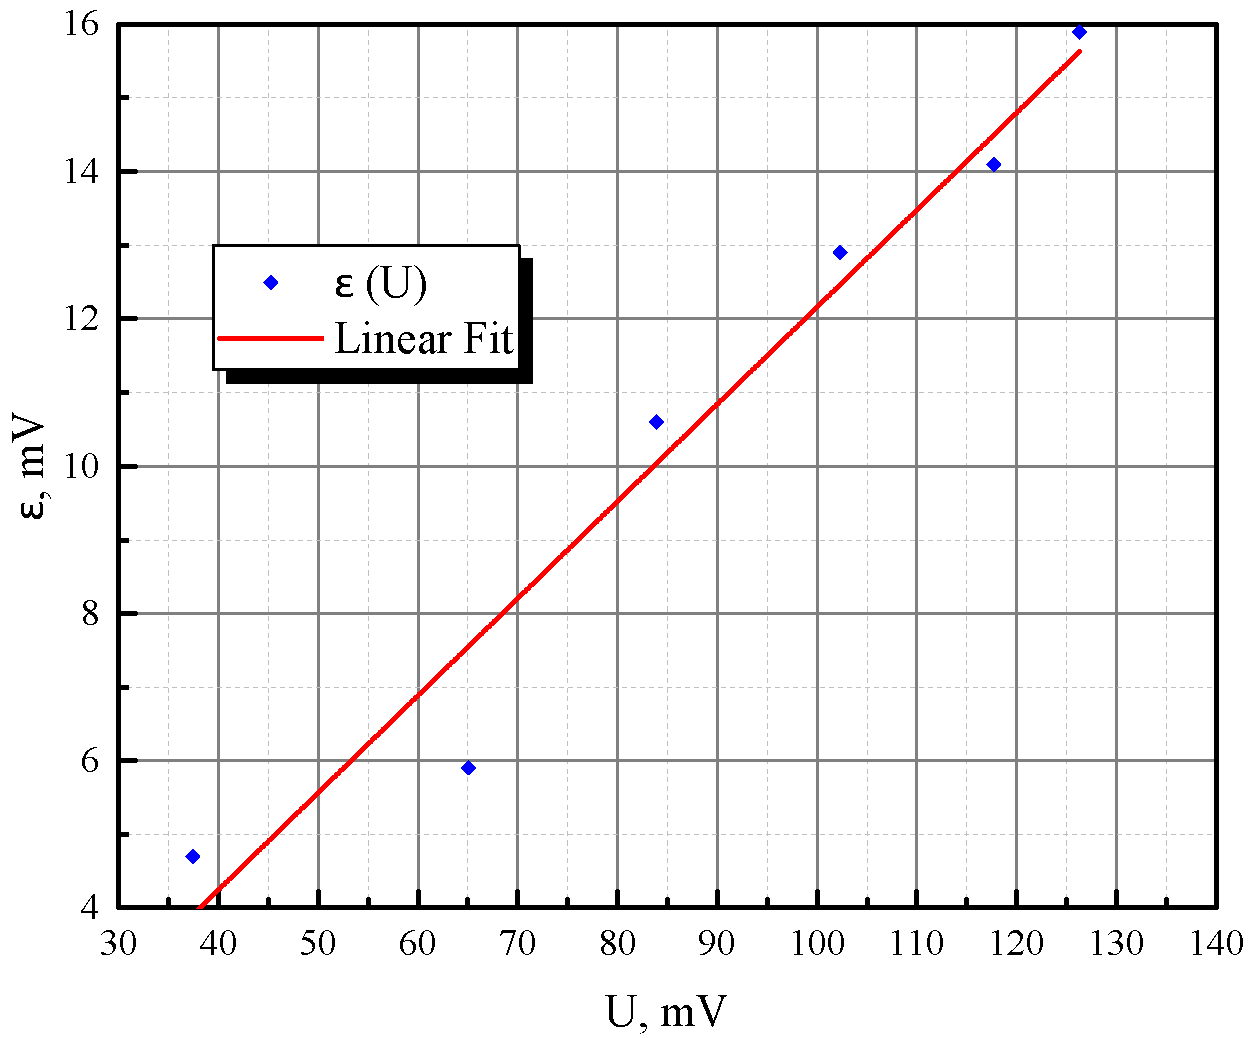
\includegraphics[width=0.7\textwidth]{img/graph.png}
    \caption{Зависимость мощности излучения от температуры в логарифмическом масштабе}
    \label{graph}
\end{figure}

Найдем величину постоянной Стефана-Больцмана для каждого измеренного значения T, превышающего 1700 K, по формуле
\begin{equation*}
    \sigma = \frac{W}{\varepsilon_T S T^4} 
\end{equation*}
Результаты представлены в таблице 2.

 \begin{table}[h]
    \centering
    \caption{Зависимость постоянной Стефана-Больцмана от термодинамической температуры}
    \label{bolts}
    \begin{tabular}{|c||c|c|c|c|c|}
 \hline
 $T$, К & 1773 & 1883 & 1998 & 2103 & 2213 
 \\
 \hline
$\varepsilon_T$ & 0,219 & 0,235 & 0,253 & 0,259 & 0,285
\\
\hline
  $\sigma, 10^{-12}$Вт/(см$^2 \cdot$ K$^4$) & 6,67 & 5,63 & 5,69 & 5,21 & 5,29
\\
\hline

\end{tabular}
\end{table}   

Усреднением получим значение $\sigma = 5,70 \pm 0,25$. Здесь погрешность складывается из среднеквадратичного отклонения при усреднении и измерительной погрешности. Полученное значение практически совпадает с теоретическим
    $\sigma_{t_h} = 5.67\cdot 10^{-12}$ Вт/(см$^2 \cdot$ K$^4$).

Оценим значение постоянной Планка:
\begin{equation*}
    h = \sqrt[3]{\frac{2 \pi^5 k_\text{Б}^4}{15 c^2 \sigma}} = (6,6 \pm 0,1) \cdot 10^{-34}\text{ Дж}\cdot\text{с}.
\end{equation*}

\subsection{Измерение яркостной температуры неоновой лампочки}
Термодинамическая температура неоновой лампочки примерно равна комнатной, что не соответствует её яркостной температуре ($\approx$ 870$^{\circ}$C). Дело в том, что неоновая лампочка в принципе не является моделью абсолютно чёрного или серого тела, и её излучение носит совершенно другую природу (переход электронов между энергетическими уровнями). То, что её свет имеет такой же цвет, что и нагретое АЧТ - совпадение.

%%%%%%%%%%%%%%%%%%%%%%%%%%%%%%%%%%%%%%%%%%%%%%%%%%%%%%%%%%%%%%%%%%%%%%%%%%%%%%%%%%%%%%%%

\section{Вывод}

В ходе работы было изучено тепловое излучение в моделях абсолютно чёрного и серого тел на примерах реальных обьектов - модели АЧТ, колец из различных материалов и вольфрамовой нити. Было проведено ознакомление с принципом работы оптического пирометра - в ходе его настройки и работы с моделью АЧТ выяснилось, что разность показаний пирометра и действительной температурой составляет до 10\%. 

При проведении работы мы наблюдали, что для различных материалов с одинаковой термодинамической температурой их яркостная температура может не совпадать. Это связано с различием коэффициента спектрального поглощения этих материалов. Также было установлено, что не все вещества излучают по законам теплового излучения, на примере неоновой лампочки.

В работе было предложено проверить справедливость закона Стефана-Больцмана ($W \propto T^4$). Полученное значения показателя степени в зависимости $W(T)$, а также значения $\sigma$ и $h$ совпали с теоретическими в пределах погрешности измерений. Это позволяет утверждать, что примененный способ исследования закономерностей теплового излучения достаточно точен. При необходимости ошибку измерения можно заметно уменьшить, если применить более точные приборы и градуировочные графики.